\subsection{State}

\begin{figure}[htb]
	\caption{\label{fig_grafico}Estrutura do State}
	\begin{center}
	    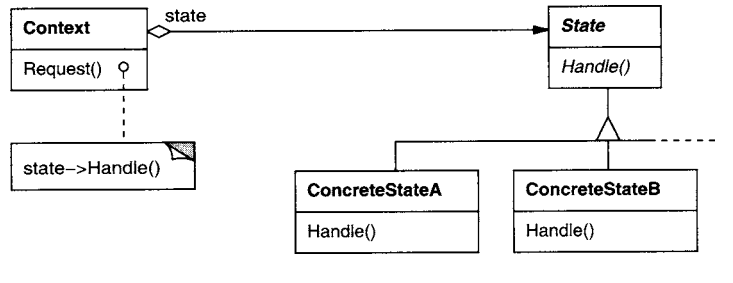
\includegraphics[scale=0.5]{5_padroes-contexto-funcional/5.3_comportamentais/5.3.08_state/diagram.png}
	\end{center}
\end{figure}

Exemplo Orientado a Objetos:

\begin{lstlisting}[caption={State Orientação a Objetos},label=oostate]


    
\end{lstlisting}

Contexto Funcional:


\begin{lstlisting}[caption={State Funcional},label=fpstate]
    

    
\end{lstlisting}